\chapter{Experiments}

\section{Deep Kalman Filter}

The notebook for the Deep Kalman Filter is 

\begin{minted}[frame=single,fontsize=\footnotesize]{python}
Train_DKF_Final.ipynb
\end{minted}

We trained the \gls{dkf} on 200 synthetic univariate time series of 100 time steps for training and 50 time steps to predict. 
The time are the sum of two sine waves with noise.

\begin{minted}[frame=single,fontsize=\footnotesize]{python}
    f1,f2,o1,o2 = np.random.rand(4, batch_size, 1)  # return 4 values for each time series
    time = np.linspace(0, 1, n_steps)  # time vector
    
    series = 0.4 * np.sin((time - o1) * (f1 * 5 + 10)) # first sine wave
    series += 0.2 * np.sin((time - o2) * (f2 * 20 + 20)) # second sine wave
    series += noise * (np.random.randn(batch_size, n_steps) - 0.5)  # add noise
\end{minted}

The training of the \gls{dkf} proved difficult, as we experienced \textbf{posterior collapse}: remember that the \gls{elbo} 
is :
\begin{align*}
    \mathcal{L}(\theta, \phi, X) &= \sum_{i=1}^n \mathbb{E}_{q_{\phi}(z_i \vert x_i)} \log{p_{\theta_x}(x_i \vert z_i)} - \sum_{i=1}^n \mathbb{KL}(q_{\phi}(z_i \vert x_i) \vert\vert p_{\theta_z}(z_i) )
\end{align*}

The posterior collapse describes the situation where the training is such that:
\begin{itemize}
    \item the posterior $q_{\phi}(z \vert x)$ becomes independent of $x$, ie $q_{\phi}(z \vert x) \approx q_{\phi}(z) \approx p_{\theta_z}(z)$
    \item the decoder is expressive enough to model the data without the latent variable: $p_{\theta_x}(x \vert z) \approx p_{\theta_x}(x)$
\end{itemize}

One way to avoid this is to introduce a $\beta$-scheduler, ie a varying weight between the $\mathbb{KL}$ term and the reconstruction term. Fisrt, $\beta=0$, 
the total loss is exclusively the reconstruction loss until it reaches a certain threshold. Then $\beta$ increases to incorporate gradually the $\mathbb{KL}$ term.

\begin{figure}[H]
    \centering
    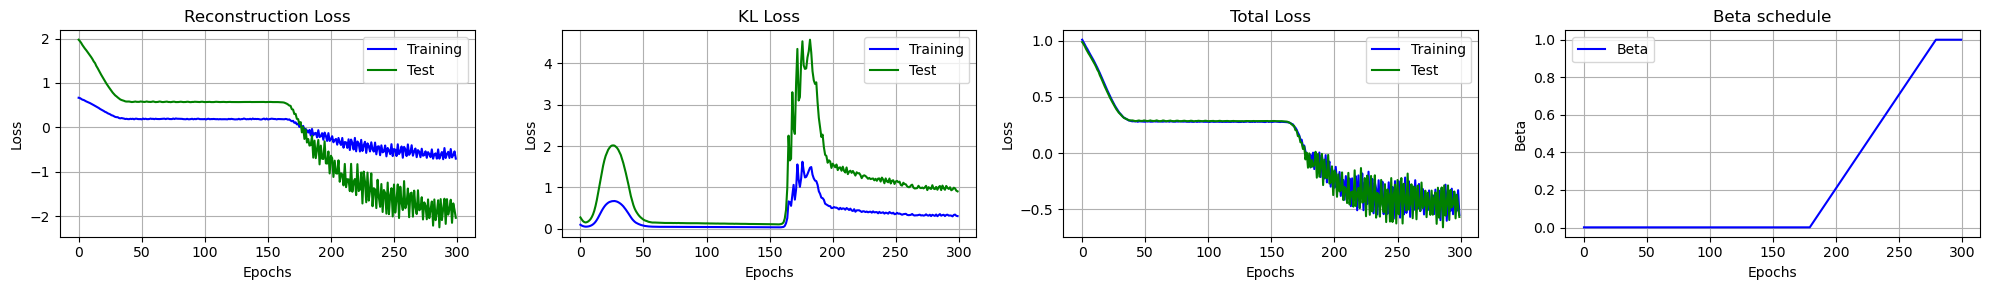
\includegraphics[width=0.9\textwidth]{/home/benjamin/Folders_Python/MVA/MVA_Stage/images/dkf_loss_courbe.png}
    \caption{Training DKF}
    \label{fig:Training DKF}
\end{figure}

The model was able to reconstruct the time-series and generates plausible predictions.

\begin{figure}[H]
    \centering
    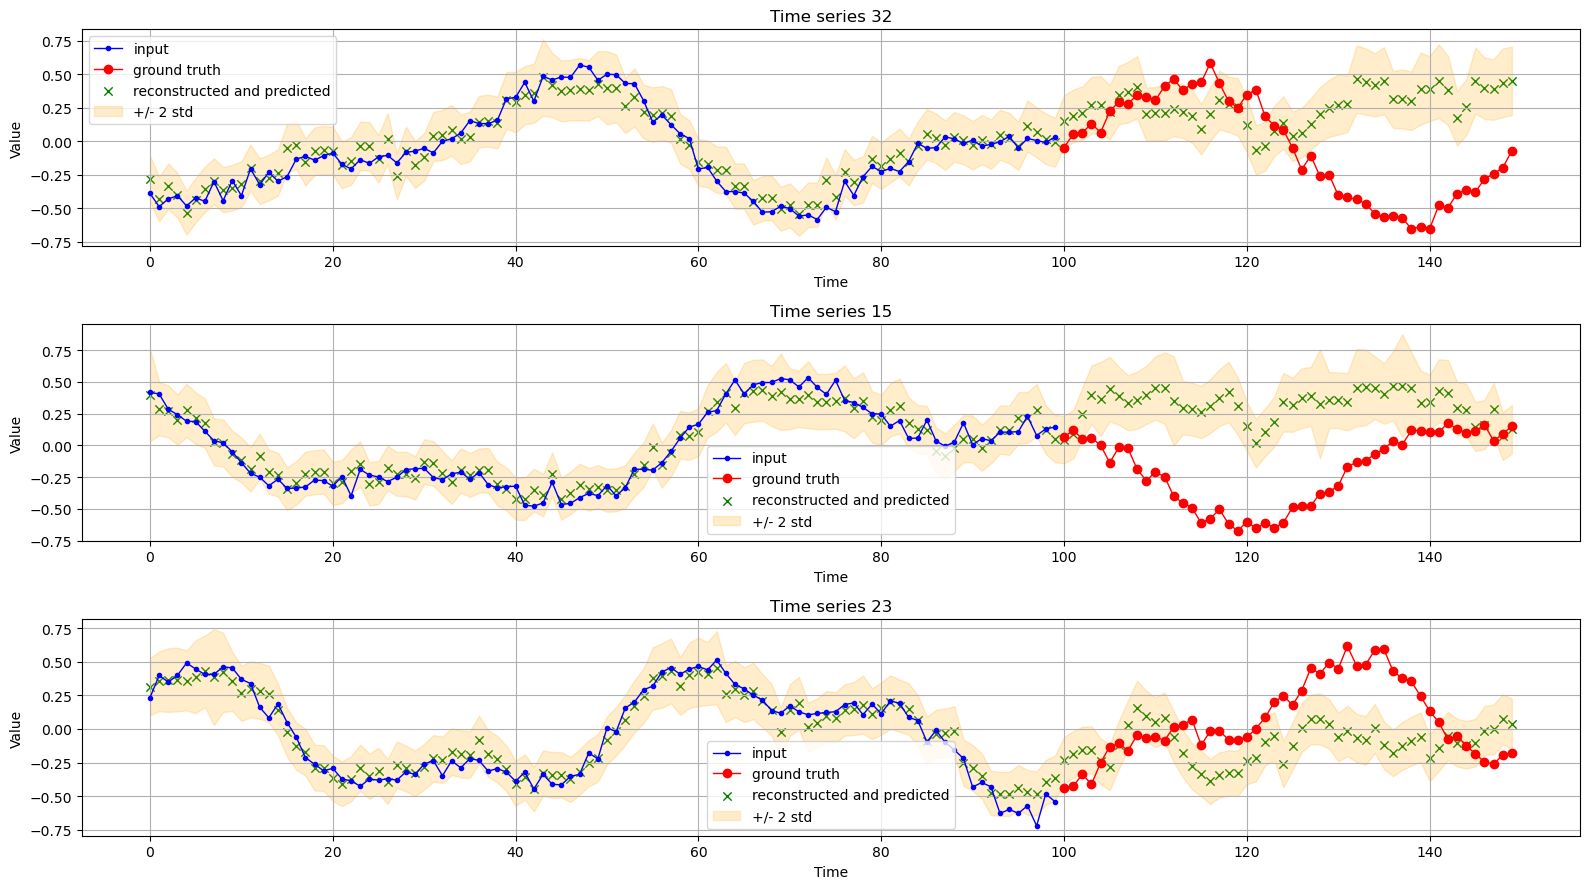
\includegraphics[width=0.9\textwidth]{/home/benjamin/Folders_Python/MVA/MVA_Stage/images/dkf_preds_gens.png}
    \caption{Predictions Generations DKF}
    \label{fig:Predictions Generations DKF}
\end{figure}

\section{Variational Recurrent Neural Network on time series}

We tested a \gls{vrnn} on a toy time serie dataset in
\begin{minted}[frame=single,fontsize=\footnotesize]{python}
Train_VRNN_v1.ipynb
\end{minted}
The time series are shorter than for the \gls{dkf} to reduce training time - thus making the task easier. Results are promising though.

\begin{figure}[H]
    \centering
    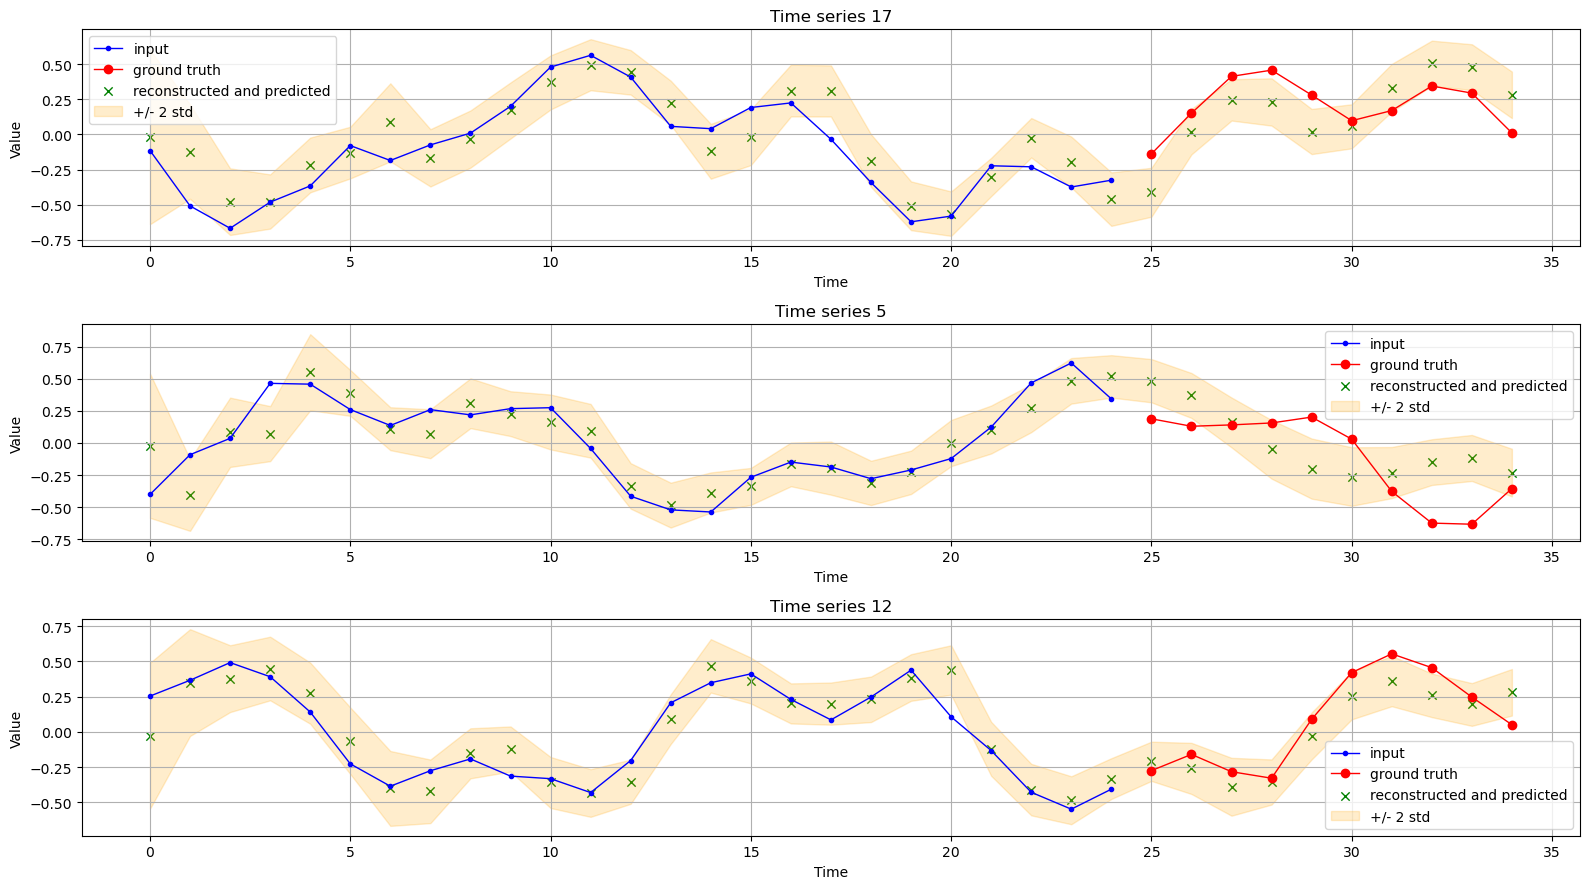
\includegraphics[width=0.9\textwidth]{/home/benjamin/Folders_Python/MVA/MVA_Stage/images/vrnn_toy_time_series.png}
    \caption{Predictions Generations VRNN}
    \label{fig:Predictions Generations VRNN}
\end{figure}


\section{Sprites Dataset}

We will be using the \textbf{Sprites} dataset from \cite{li_disentangled_2018}.

The Sprites dataset is a synthetic cartoon character dataset of RGB images $64 \times 64 \times 3$. Each character has 4 attributes 
(hair, shoes, top cloth, bottom cloth) that can take 6 possibles values. Each character has three possible poses (left, front, right) 
and can perform 3 possible actions (walk, spell, slash) accross 8 consecutive frames.

There is a total of $6^4 \times 3 \times 3 = 11664$ series of 8 images each, that are divided between a training set and a 
test set.

Here is one character:
\begin{figure}[H]
    \centering
    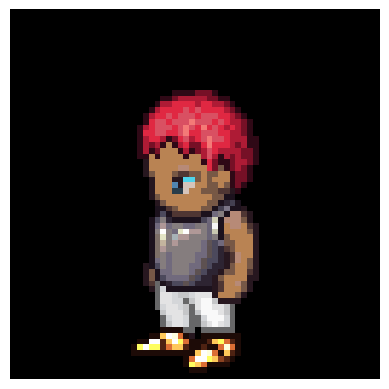
\includegraphics[width=0.4\textwidth]{/home/benjamin/Folders_Python/MVA/MVA_Stage/images/one_sprite.png}
    \caption{One sprite}
    \label{fig:One sprite}
\end{figure}

And 5 series:
\begin{figure}[H]
    \centering
    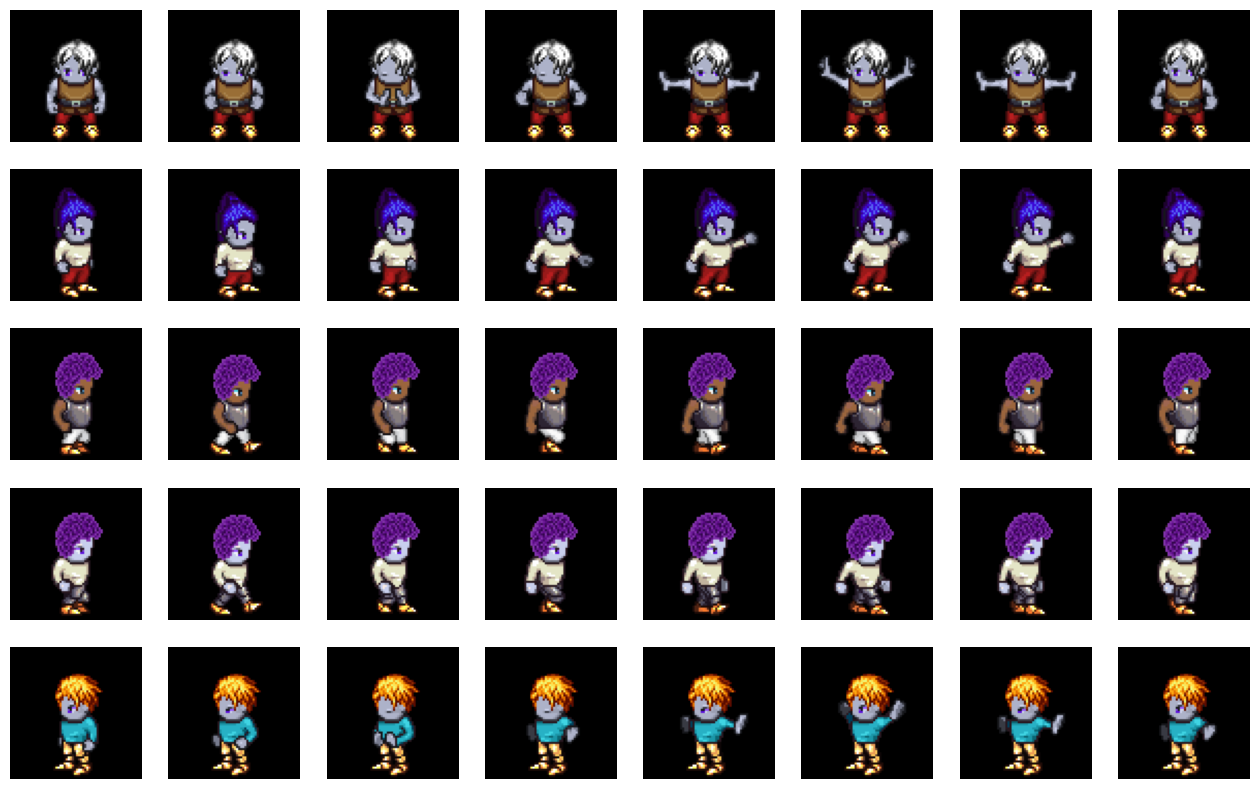
\includegraphics[width=0.9\textwidth]{/home/benjamin/Folders_Python/MVA/MVA_Stage/images/samples_sprites_series.png}
    \caption{sprite series}
    \label{fig:sprite series}
\end{figure}

\section{Variational Recurrent Neural Network}

We trained a \gls{vrnn} in
\begin{minted}[frame=single,fontsize=\footnotesize]{python}
Train_VRNN_Sprites_v1.ipynb
\end{minted}
with a CNN encoder and a CNN decoder. 
The three RNNs of the \gls{vrnn} have a dimension 128, and the latent space dimension is 64.

The training took a little bit more than one hour on a RTX 3090.

The reconstruction is good

\begin{figure}[H]
    \centering
    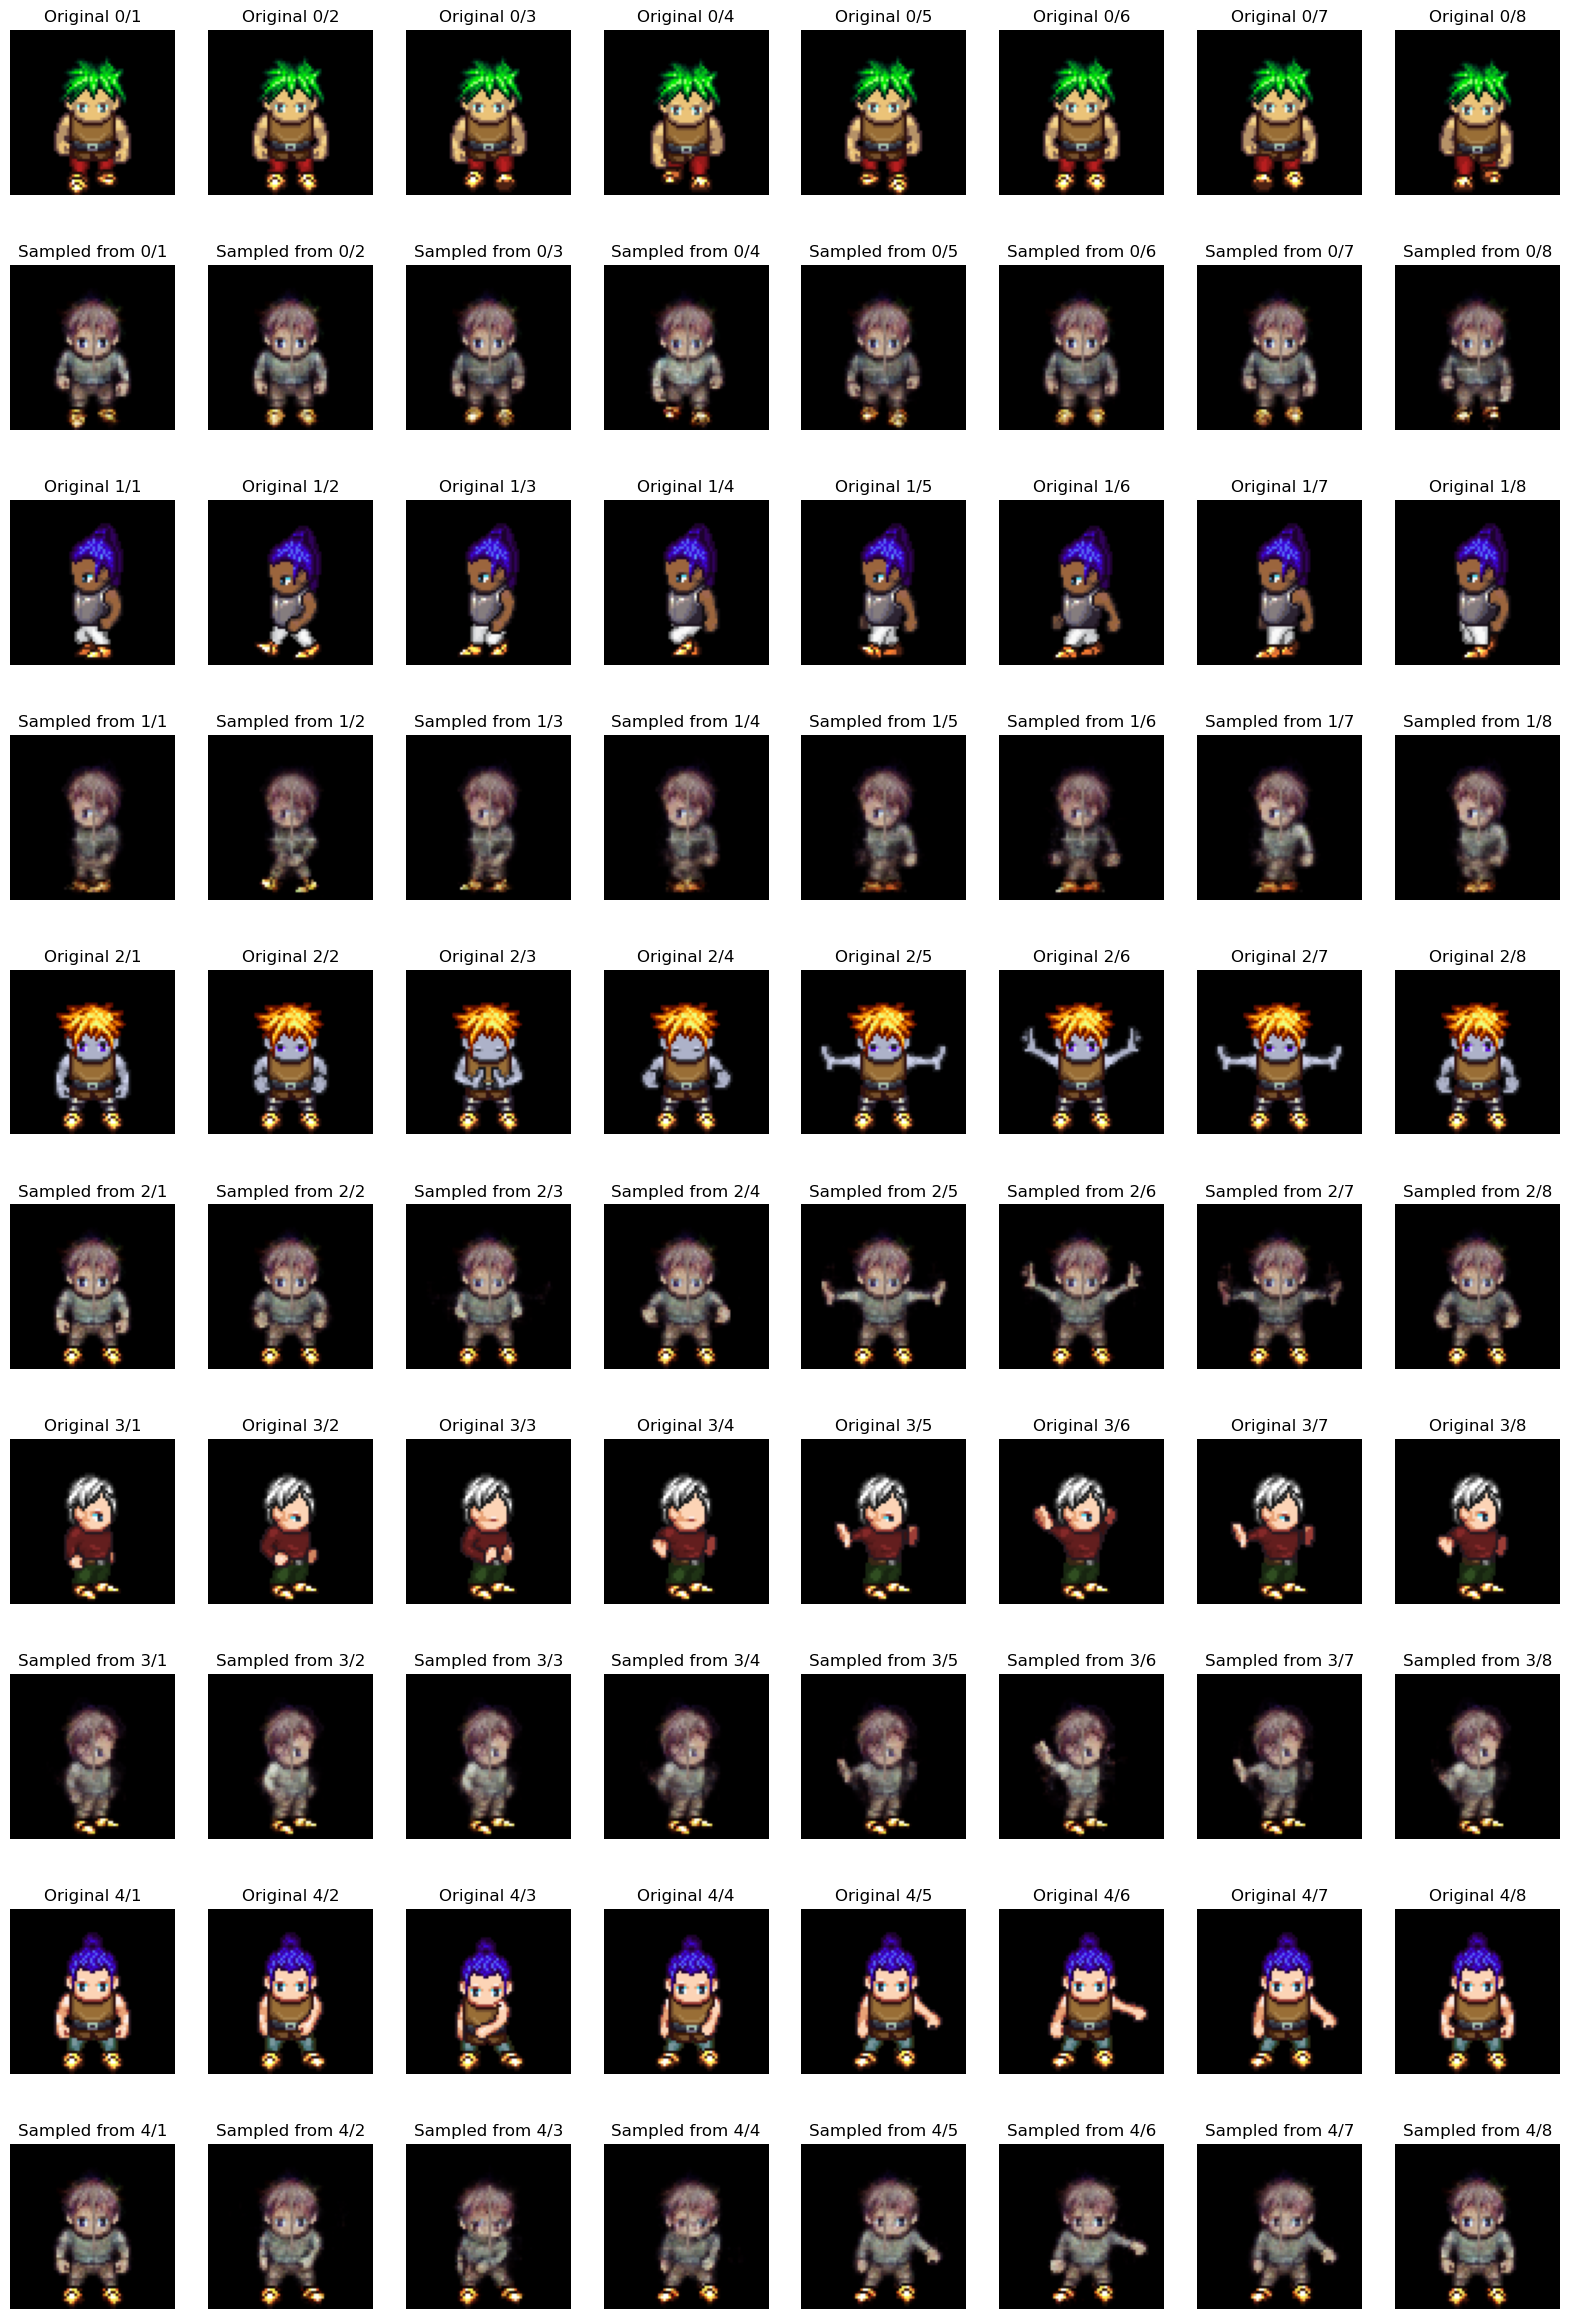
\includegraphics[width=0.9\textwidth]{/home/benjamin/Folders_Python/MVA/MVA_Stage/images/vrnn_sprites_reconstruction.png}
    \caption{VRNN Sprites reconstruction}
    \label{fig:VRNN Sprites reconstruction}
\end{figure}

\newpage
\begin{landscape}
We tested the generation over 20 time steps, with one character as a "seed" to intialize the first latent variable. The model 
can sometimes chain different motions over those 20 steps.

\begin{figure}[H]
    \centering
    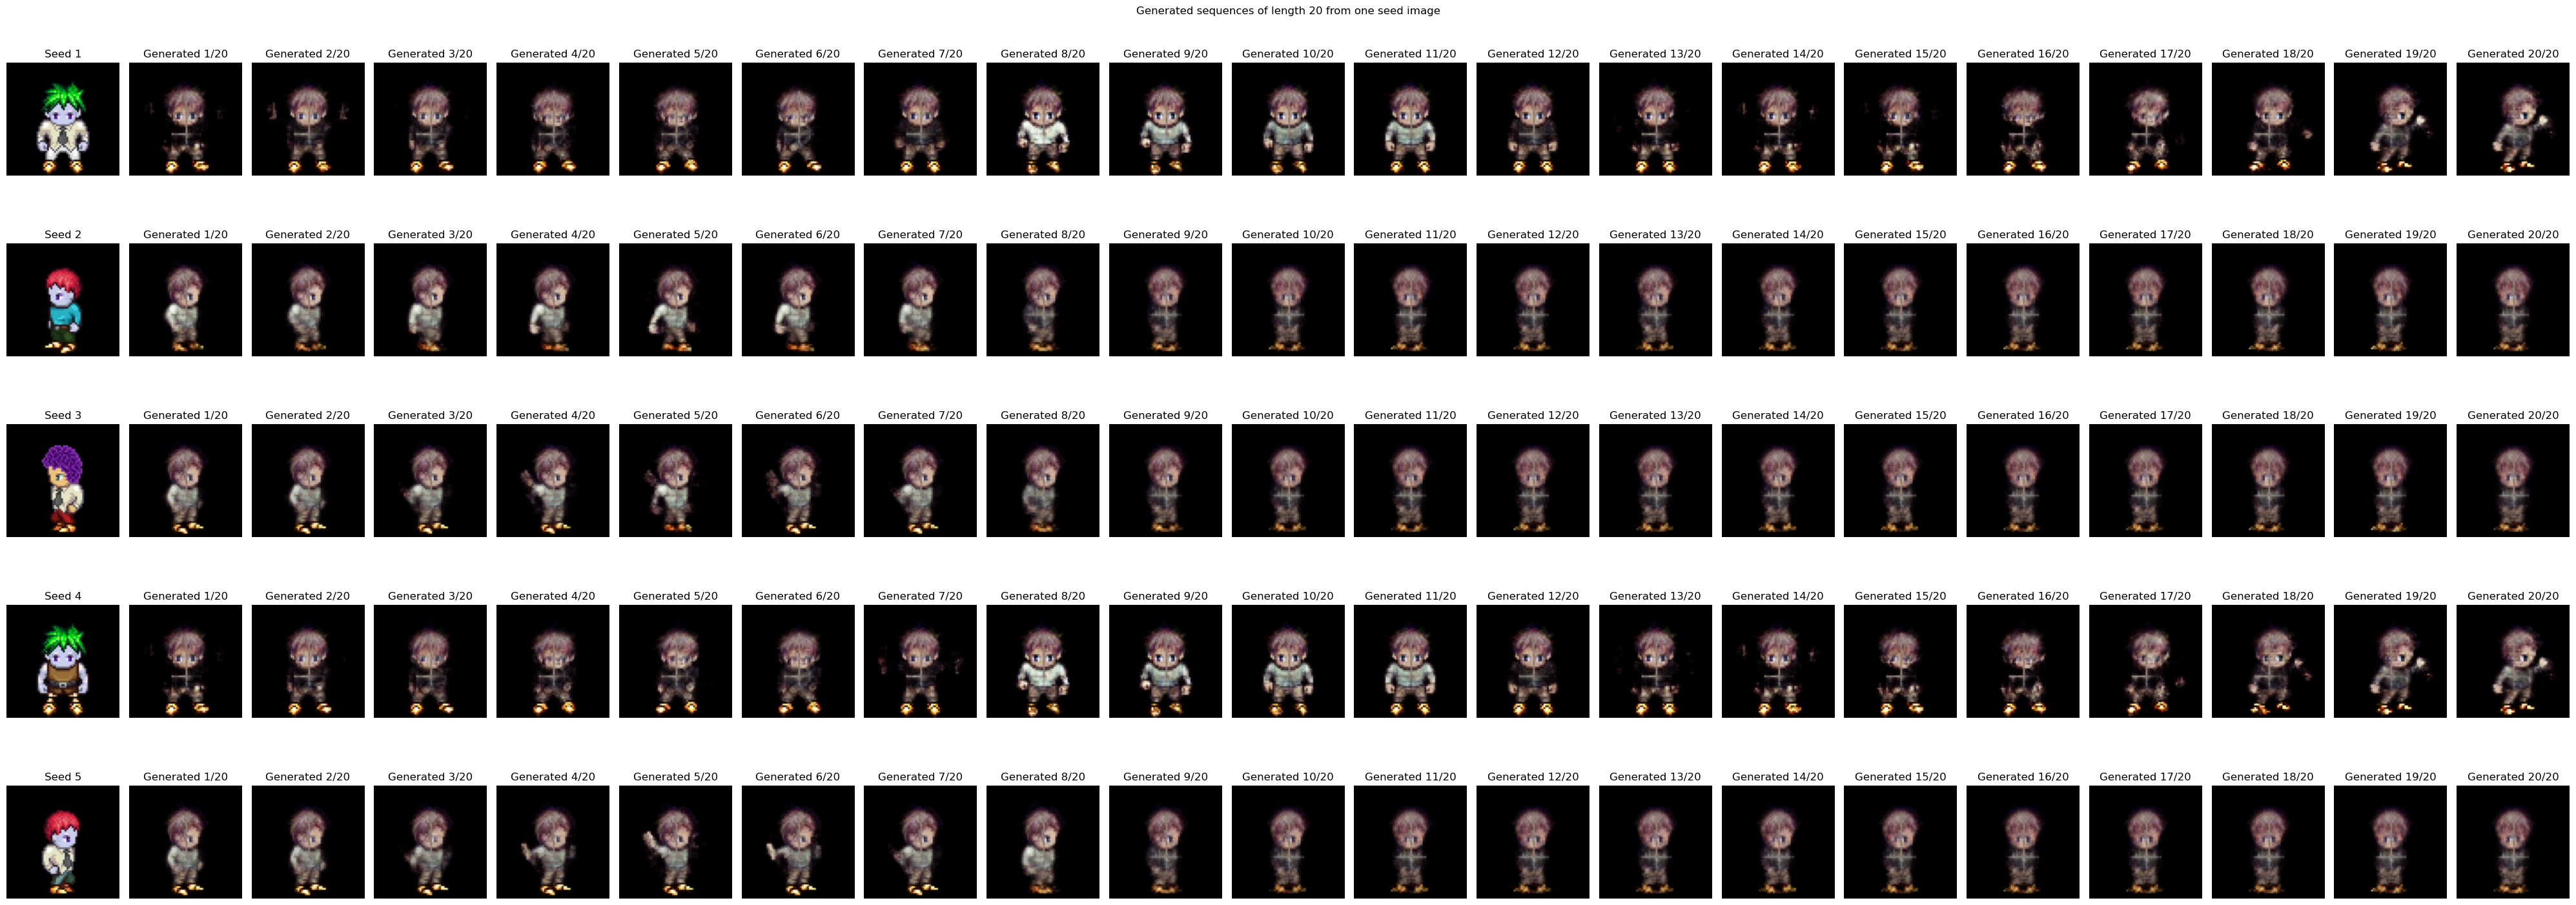
\includegraphics[width=1.3\textwidth]{/home/benjamin/Folders_Python/MVA/MVA_Stage/images/vrnn_sprites_generation.png}
    \caption{VRNN Sprites generation}
    \label{fig:sprite generation}
\end{figure}
\end{landscape}

\section{Gaussian Process Variational Auto Encoder}

The training of the \gls{gpvae} proved challenging.

See the detailed training logic in:
We trained a \gls{vrnn} in
\begin{minted}[frame=single,fontsize=\footnotesize]{python}
Train_GPVAE_step_by_step_logic.ipynb
\end{minted}

The specific notebook for the sprite training is 
\begin{minted}[frame=single,fontsize=\footnotesize]{python}
Train_GPVAE_Sprites_XPs_v2.ipynb
\end{minted}

We coded three different ways of computing a covariance matrix:
\begin{itemize}
    \item covariance matrix
    \item precision matrix
    \item Cholesky decomposition
\end{itemize}

We coded Gaussian kernels and Matern kernels (with $\nu = 0.5, 1.5, 2.5$).
The \mint{python3}|class GaussianKernelFixed| and \mint{python3}|class MaternKernelFixed| have fixed non-trainable lengthscale 
and sigma parameters (sigma is the scaling factor multiplying the kernel).

The \mint{python3}|class GaussianKernel| and \mint{python3}|class MaternKernel| have learnable lengthscale 
and sigma parameters : 
\begin{minted}[frame=single,fontsize=\footnotesize]{python}
self.lengthscale = nn.Parameter(torch.tensor(lengthscale))  # learnable lengthscale parameter    
self.sigma = nn.Parameter(torch.tensor(sigma))  # learnable variance parameter
\end{minted}
However, the attributes must be cloned before being used in the computations to avoid running multiple backward passes in the 
computation graph ... :
\begin{minted}[frame=single,fontsize=\footnotesize]{python}
lengthscale = self.lengthscale.clone()
sigma = self.sigma.clone()
# ...
kernel = torch.exp(-0.5 * torch.pow(torch.div(t1_b - t2_b, lengthscale),2))  # (..., N, M)
# ...        
gaussian_kernel_matrix = sigma**2 * kernel
\end{minted}

After several tests, we used a total of 32 \glspl{gp} priors of the 4 different kernel types, with different lengthscales:
\begin{minted}[frame=single,fontsize=\footnotesize]{python}
Dz = 32
delta_t = 1.0  # time step between two frames if T=8 frames in [0,1]

kernels_list = [ GaussianKernelFixed(lengthscale=(delta_t / (2**i)), sigma=1.0).to(device) 
for i in range(int(Dz/4)) ] + \
[ MaternKernelFixed(nu=0.5, lengthscale=(delta_t / (2**i)), sigma=1.0).to(device) 
for i in range(int(Dz/4)) ] +  \
[ MaternKernelFixed(nu=1.5, lengthscale=(delta_t / (2**i)), sigma=1.0).to(device) 
for i in range(int(Dz/4)) ] + \
[ MaternKernelFixed(nu=2.5, lengthscale=(delta_t / (2**i)), sigma=1.0).to(device) 
for i in range(int(Dz/4)) ]

mean_functions_list = [ GPNullMean().to(device) for _ in range(Dz) ] # list of Dz identical mean functions
mean, kernel_matrix, L_matrix, p_theta_z = compute_gp_priors(t, Dz, kernels_list, mean_functions_list, 
verbose=True)
\end{minted}

The reconstruction is good without being perfect:
\begin{figure}[H]
    \centering
    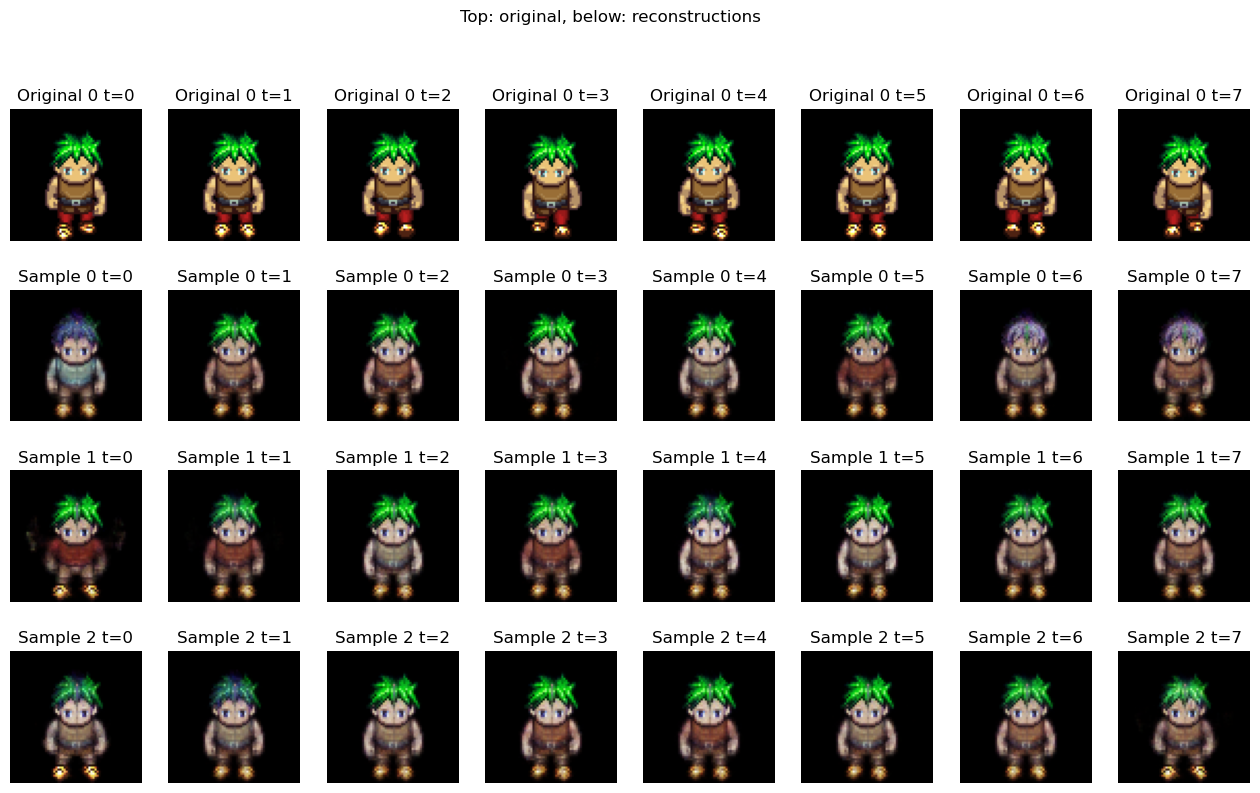
\includegraphics[width=0.9\textwidth]{/home/benjamin/Folders_Python/MVA/MVA_Stage/images/gpvae_reco_01.png}
    \caption{GPVAE Sprites reconstruction 1}
    \label{fig:GPVAE Sprites reconstruction 1}
\end{figure}

\begin{figure}[H]
    \centering
    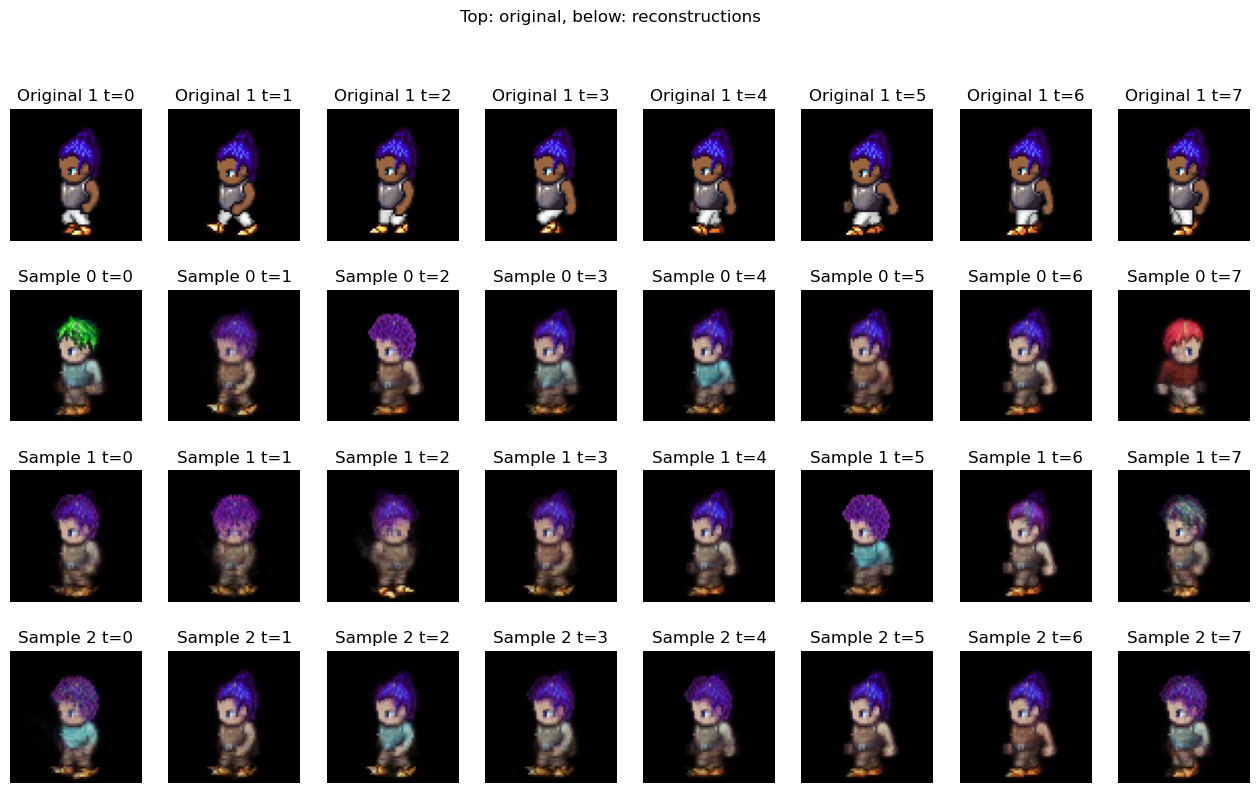
\includegraphics[width=0.9\textwidth]{/home/benjamin/Folders_Python/MVA/MVA_Stage/images/gpvae_reco_02.png}
    \caption{GPVAE Sprites reconstruction 2}
    \label{fig:GPVAE Sprites reconstruction 2}
\end{figure}

\begin{figure}[H]
    \centering
    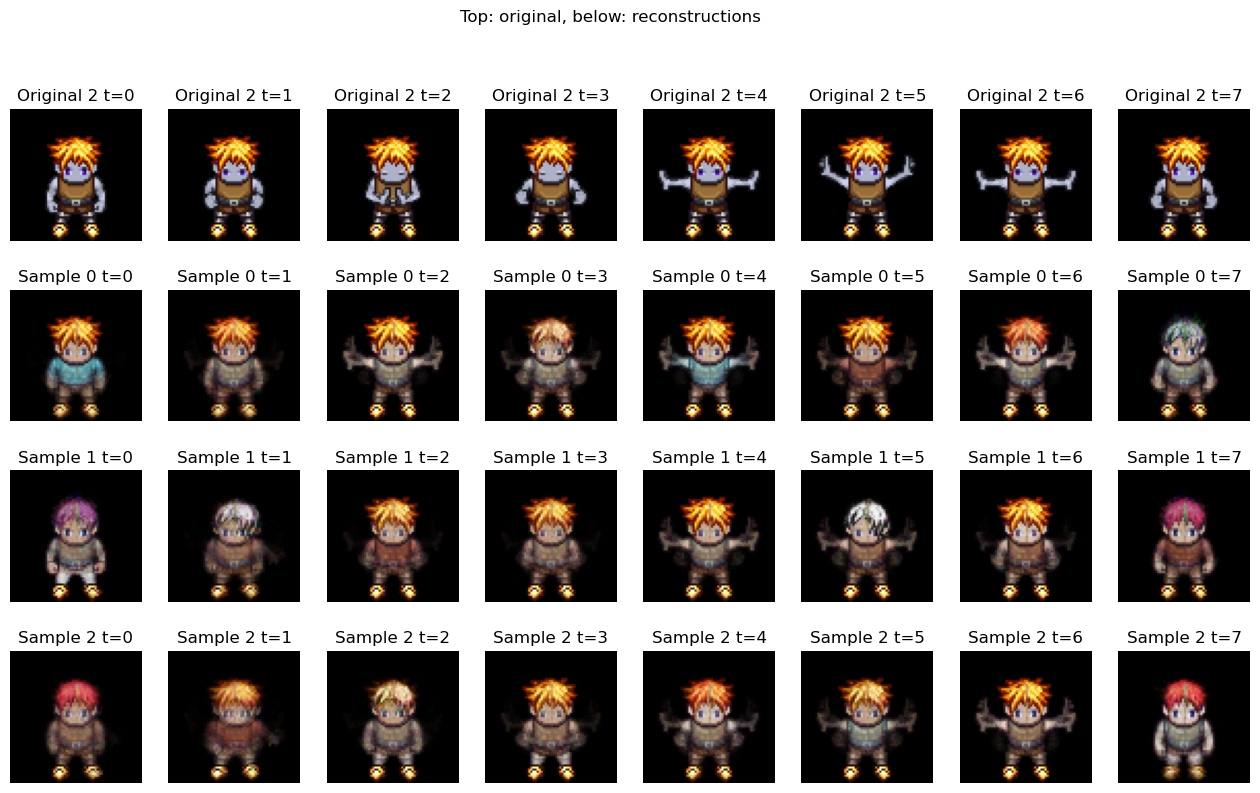
\includegraphics[width=0.9\textwidth]{/home/benjamin/Folders_Python/MVA/MVA_Stage/images/gpvae_reco_03.png}
    \caption{GPVAE Sprites reconstruction 3}
    \label{fig:GPVAE Sprites reconstruction 3}
\end{figure}

The generation is not perfect yet!

\begin{figure}[H]
    \centering
    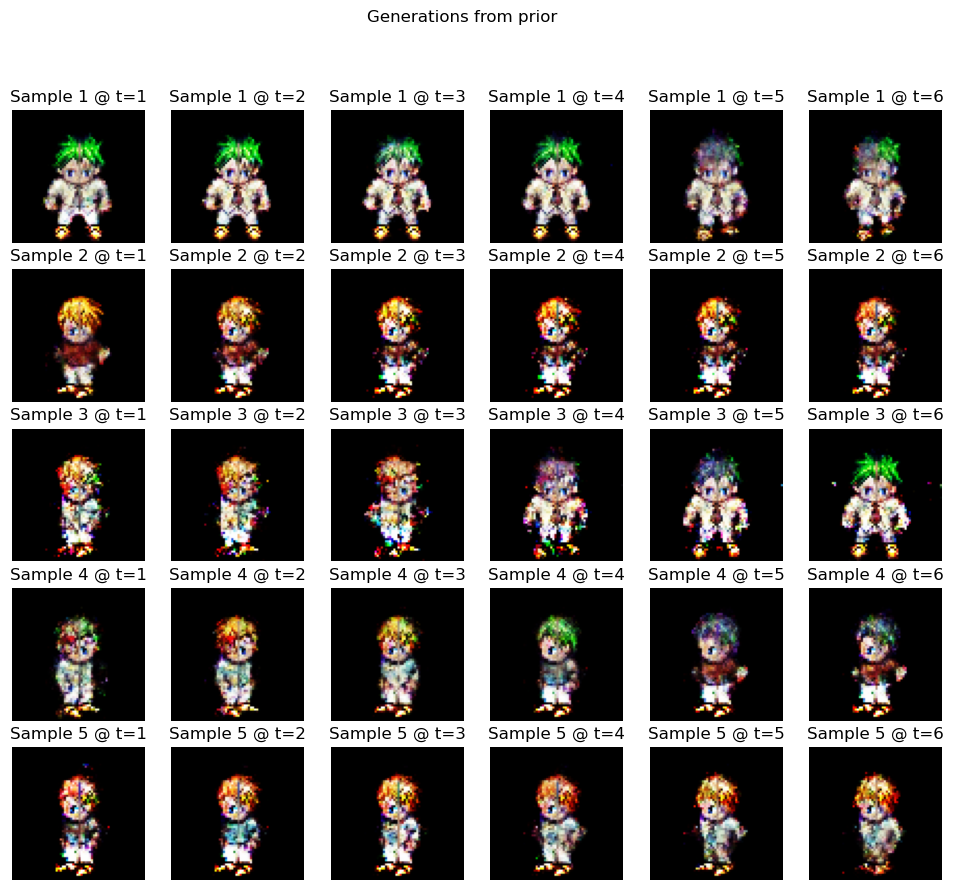
\includegraphics[width=0.9\textwidth]{/home/benjamin/Folders_Python/MVA/MVA_Stage/images/gpvae_gen_01.png}
    \caption{GPVAE Sprites generation 1}
    \label{fig:GPVAE Sprites generation 1}
\end{figure}